\documentclass{beamer}
\usetheme{Warsaw}

\usepackage[utf8]{inputenc}
\usepackage{fancybox}
\usepackage{multimedia} 
\usepackage{subfig}
\usepackage{amsmath}
\usepackage{hyperref}
\usepackage[all]{xy}
\usepackage{algorithm}
\usepackage[noend]{algpseudocode}

\begin{document}


\title[Angewandte Mathematik] % (optional, only for long titles)
{Angewandte Mathematik
\\
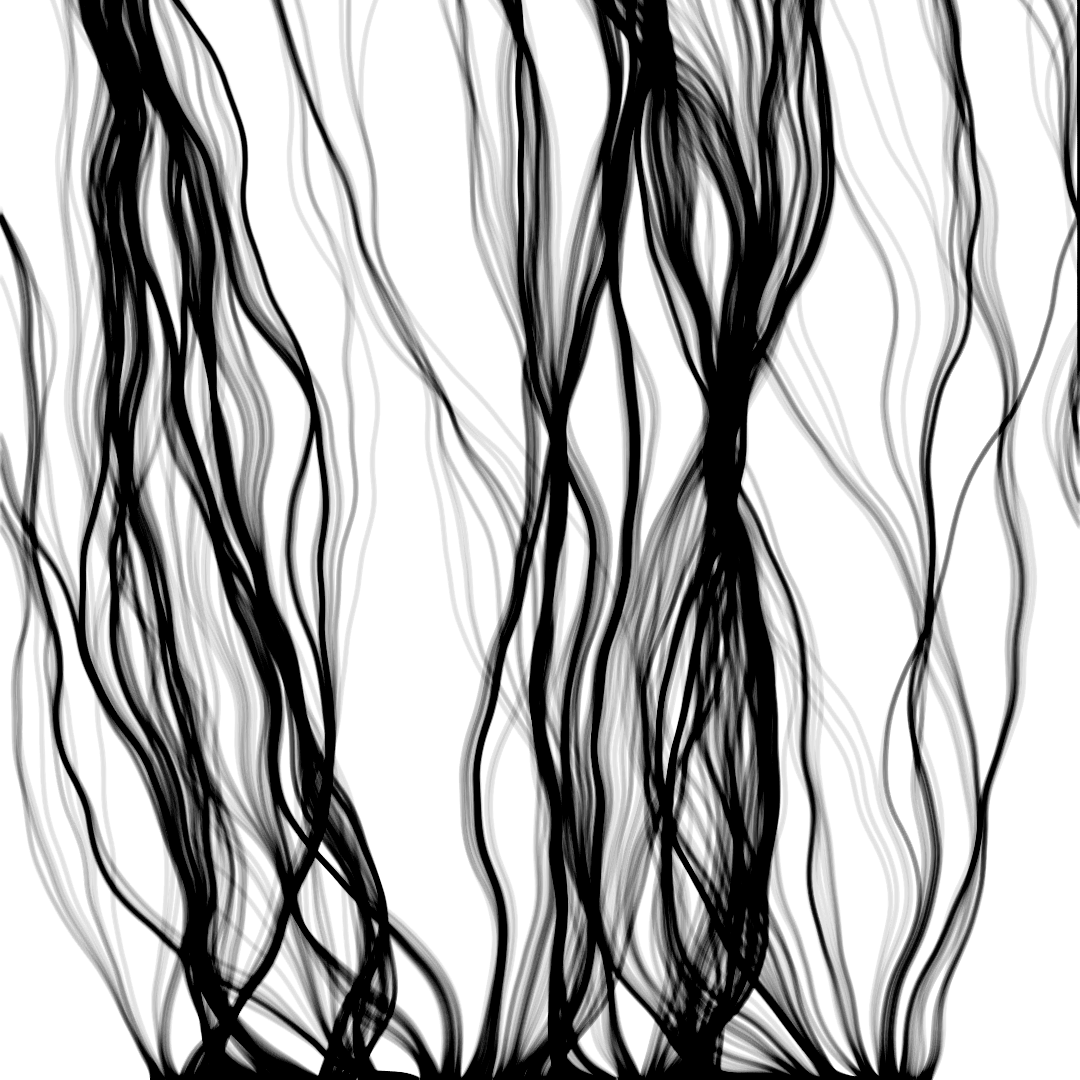
\includegraphics[scale=0.15]{images/cover}
}
\subtitle{}
\author[Dr. Johannes Riesterer] % (optional, for multiple authors)
{Dr.  rer. nat. Johannes Riesterer}

\date[KPT 2004] % (optional)
{}

\subject{Angewandte Mathematik}



\frame{\titlepage}




\begin{frame}
    \frametitle{Angewandte Mathematik}
\framesubtitle{Gradientenverfahren}
    \begin{block}{Gradientenverfahren}
Wie kann man Minima einer  differenzierteren Abbildung $f: \mathbb{R}^n \to \mathbb{R}$ finden? 
 
\end{block}

    \begin{block}{Gradientenverfahren}
\begin{itemize}
\item An jedem Punkt $x_k \in  \mathbb{R}^n$ zeigt der negative Gradient  $d_k := -\nabla f (x_k)$ in die steilste Abstiegsrichtung.
\item Für hinreichend kleines $\alpha_k$ folgt mit Satz über die lokale Liberalisierung  
$f(x_{k+1}) = f (x_k + \alpha_k d_k) =  f(x_k) + \alpha_k df(x_k)d_k + R( \alpha_k dk)$
\item  Setze $x_{k+1} = x_k + \alpha_k d_k$ 
\item Es gilt $f(x_{k+1}) \leq f(x_k)$, falls $\nabla f(x_k) \neq 0$
\item  Falls die folge $f(x_k)$ beschränkt ist, so ist  dieser Fixpunkt $x^*$ ein minimum, da $\nabla f(x^*) = 0$ gelten muss.  
\end{itemize}

\end{block}
 \end{frame}



\begin{frame}
    \frametitle{Angewandte Mathematik}
\framesubtitle{Gradientenverfahren}
\begin{figure}[H]
      \centering
    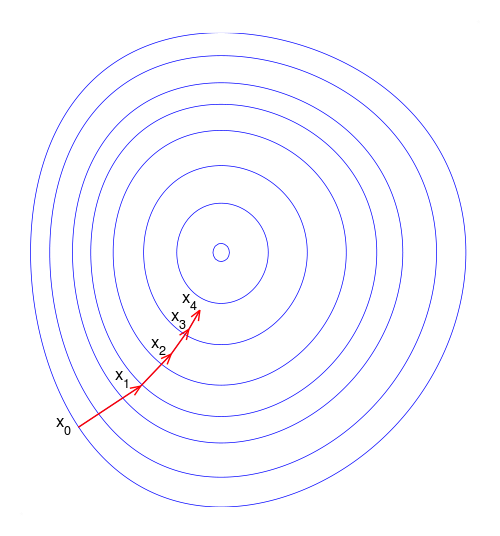
\includegraphics[width=0.5\textwidth]{images/Gradient_descent}
      \caption{Quelle: Wikipedia}
\end{figure}

 \end{frame}




\begin{frame}
    \frametitle{Angewandte Mathematik}
\framesubtitle{Gradientenverfahren}
    \begin{block}{Höhenlineien}
Sei  $f: \mathbb{R}^n \to \mathbb{R}$  eine differenzierbare Funktion. Eine Kurve $\gamma : I \to \mathbb{R}^n$, auf der $f$ konstant ist, also 
$f(\gamma(t)) = c$ für eine festes $c \in \mathbb{R}$ gilt, heißt Höhenlinie.
\end{block}

\begin{figure}[H]
      \centering
    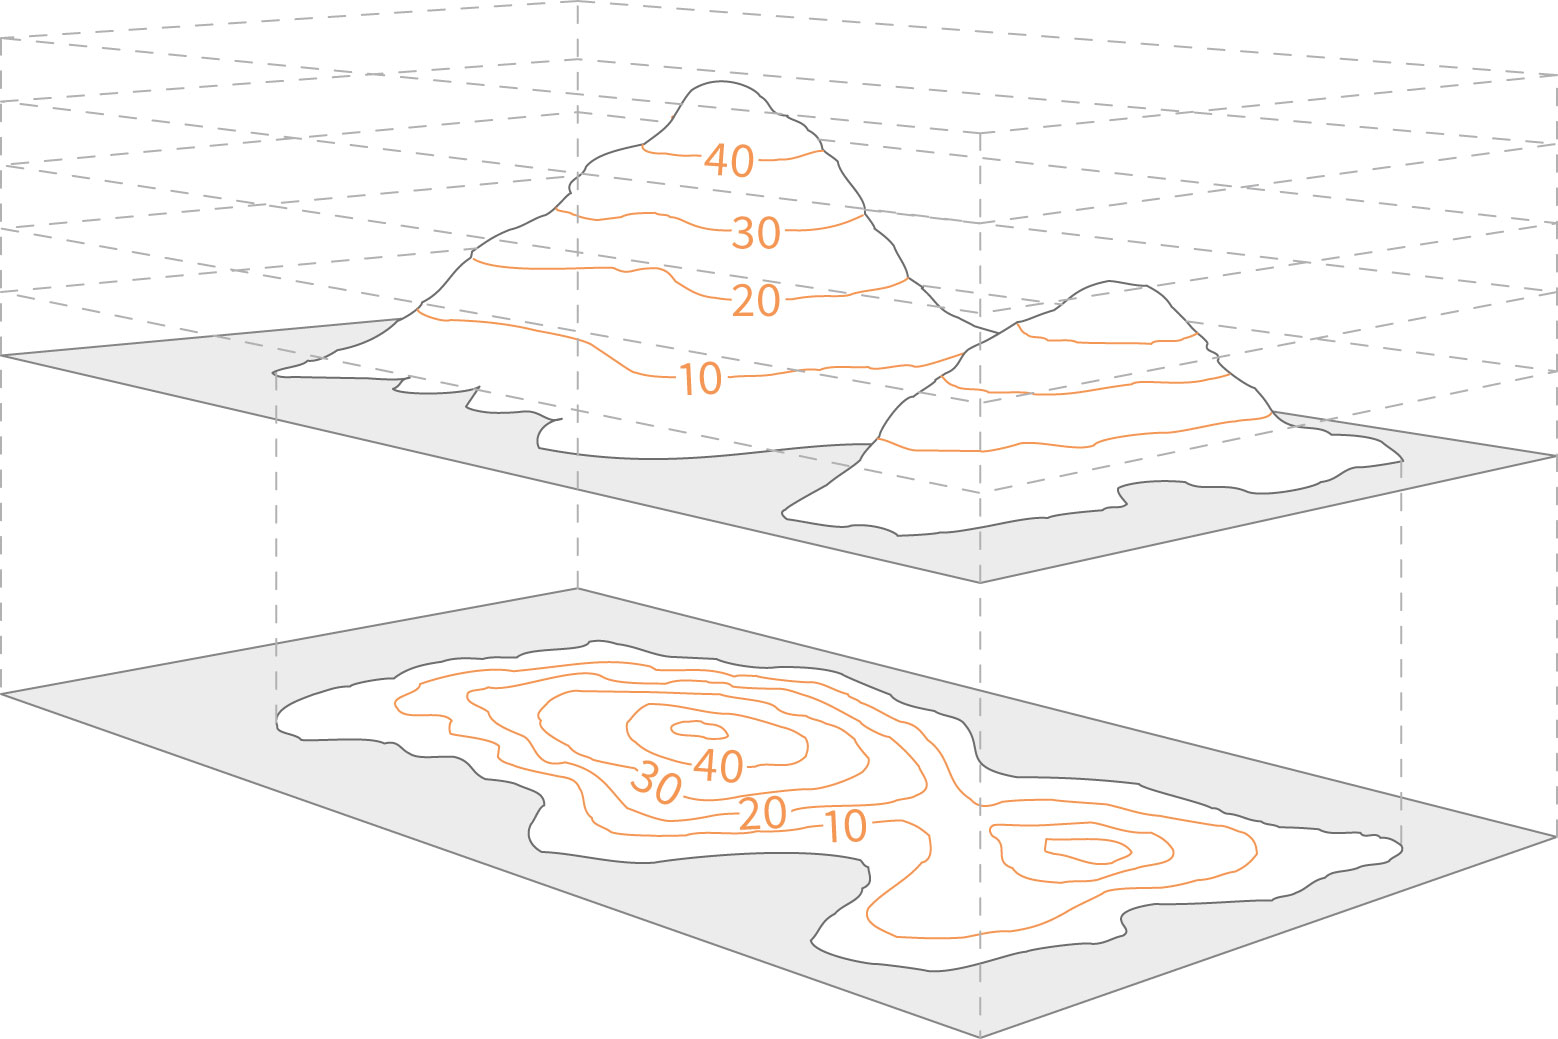
\includegraphics[width=0.5\textwidth]{images/Contours-and-relief}
      \caption{Quelle: https://getoutside.ordnancesurvey.co.uk/guides/understanding-map-contour-lines-for-beginners/}
\end{figure}

 \end{frame}


\begin{frame}
    \frametitle{Angewandte Mathematik}
\framesubtitle{Gradientenverfahren}
    \begin{block}{Höhenlineien}
Der Gradient steht senkrecht auf  Höhenlinien. Dies bedeutet, dass $$ \bigl \langle \nabla f(\gamma(t)), \gamma'(t) \bigr \rangle = 0$$ gilt. 

\end{block}
    \begin{block}{Beweis}
Aus $f(\gamma(t)) = c$ folgt $\frac{d}{dt} f(\gamma(t)) = 0$. Mit der Kettenregel folgt $\frac{d}{dt} f(\gamma(t)) =  f(\gamma(t)) \cdot \gamma'(t) = 0$ und damit
$ \bigl \langle \nabla f(\gamma(t)), \gamma'(t) \bigr \rangle = 0$.
\end{block}

 \end{frame}



\begin{frame}
    \frametitle{Angewandte Mathematik}
\framesubtitle{Backpropagation}
    \begin{block}{Backpropagation}
Das Gradientenverfahren angewendet auf eine Lossfunktion eines neuronalen Netzes wird als Backpropagation bezeichnet.
Gegeben ist ein neuronales Netz $f : \Omega \times \mathbb{R}^n \to \mathbb{R}^m$, 
und ein  Datensatz $D : = \{ (x_i, y_i) \}$. Finde Gewichte Omega, so dass Lossfunktion
\begin{align*}
L_D  : \Omega \subset \mathbb{R}^n \to \mathbb{R} 
\end{align*}
minimal wird. Zum Beispiel $$L_D(\omega) := \sum_{(x_i,y_i) \in D} (f(\omega, x_i) - y_i)^2$$.

\end{block}
 \end{frame}


\begin{frame}
    \frametitle{Angewandte Mathematik}
\framesubtitle{Backpropagation}
 \begin{figure}[!tbp]
  \centering
  \begin{minipage}[b]{0.45\textwidth}
    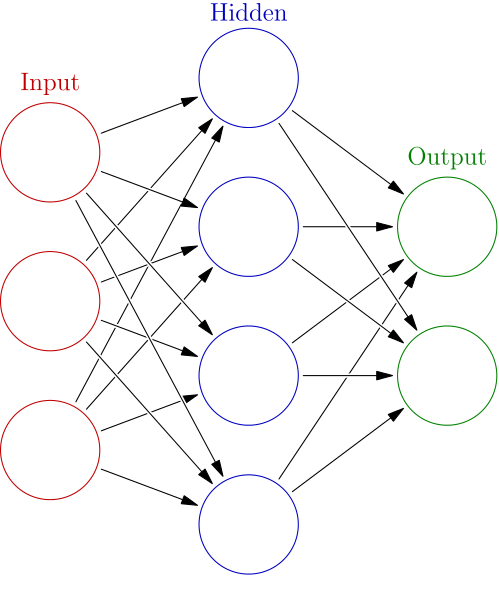
\includegraphics[width=0.6\textwidth]{images/499px-Colored_neural_network}
    \caption{Grobe Überdeckung}
  \end{minipage}
  \hfill
  \begin{minipage}[b]{0.45\textwidth}
    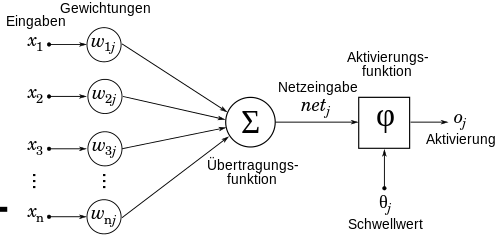
\includegraphics[width=1.0\textwidth]{images/500px-NeuronModel_deutsch}
    \caption{Feinere Überdeckung}
  \end{minipage}
\end{figure}
 \end{frame}


\begin{frame}
    \frametitle{Angewandte Mathematik}
\framesubtitle{Backpropagation}
    \begin{block}{Backpropagation}
\begin{itemize}
\item  Initialisiere $k:=0$ und zufällige Gewichte $w_0$.
\item \pause Initialisiere Genauigkeit $\epsilon > 0$
\item \pause   \text{While } {$|| \nabla L_D(\omega) || > \epsilon$}  
\item \pause Bestimme $\alpha_k$  mit $ L_D(\omega_k + \alpha d_k) =  L_D(\omega_k) + \alpha_k d L_D(\omega_k)d_k + R( \alpha_k dk)$ 
\item \pause  Setze $\omega_{k+1} := \omega_k  + \alpha_k d_k$. 
\item \pause $k \leftarrow k+1$
\end{itemize}
\end{block}
 \end{frame}

\begin{frame}
    \frametitle{Angewandte Mathematik}
\framesubtitle{Backpropagation}
    \begin{block}{Mini Batch}
\begin{itemize}
\item   Datensatz $D$ sehr groß ist (Big Data)
\item \pause Berechnung des Gradient der Lossfunktion entsprechend aufwendig. 
\item \pause Wende Backpropagation auf Teilräume $D' \subset D$ an. (Minibatch).
\item \pause $\#D' = 1$ stochastischer Gradientenabstieg.
\end{itemize}

\end{block}
 \end{frame}



\begin{frame}
    \frametitle{Angewandte Mathematik}
\framesubtitle{Minibatch}
\begin{figure}[H]
      \centering
    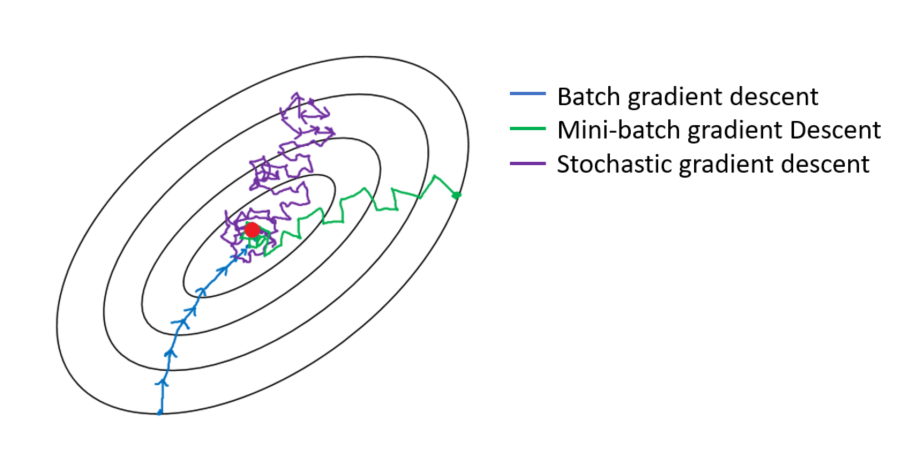
\includegraphics[width=1.0\textwidth]{images/batchgradient}
      \caption{Quelle: https://towardsdatascience.com/batch-mini-batch-stochastic-gradient-descent-7a62ecba642a}
\end{figure}

 \end{frame}
\begin{frame}
    \frametitle{Angewandte Mathematik}
\framesubtitle{Backpropagation}
    \begin{block}{Backpropagation}
\begin{itemize}
\item  Initialisiere $k:=0$ und zufällige Gewichte $w_0$.
\item \pause Initialisiere Genauigkeit $\epsilon > 0$
\item \pause Wähle Teilmenge $D_0' \subset D$
\item \pause   \text{While } {$|| \nabla L_{D_k'}(\omega) || > \epsilon$}  
\item \pause Bestimme $\alpha_k$  mit $ L_{D_k'}(\omega_k + \alpha d_k) =  L_{D_k'}(\omega_k) + \alpha_k d L_{D_k'}(\omega_k)d_k + R( \alpha_k dk)$ 
\item \pause  Setze $\omega_{k+1} := \omega_k  + \alpha_k d_k$. 
\item \pause Wähle neue Teilmenge $D'_{k +1} \subset D$.
\item \pause $k \leftarrow k+1$
\end{itemize}
\end{block}
 \end{frame}



\begin{frame}
    \frametitle{Angewandte Mathematik}
\framesubtitle{Ableitung mehrdimensionale Funktionen }
    \begin{block}{Gradient einer  mehrdimensionalen Funktion}
Eine Funktion $F: U \to \mathbb{R}^m$ heißt differenzierbar, wenn es eine lineare Abbildung $dF$ gibt, so dass 
\begin{align*}
F(a + h) = F(a) + dF(a)h + R(h)
\end{align*}
mit $\lim_{h \to 0} \frac{R(h)}{||h||} = 0$ gilt für alle $a \in U$ und $h \in \mathbb{R}^n$.
\end{block}
 \end{frame}


\begin{frame}
    \frametitle{Angewandte Mathematik}
\framesubtitle{ Ableitung mehrdimensionale Funktionen}
    \begin{block}{Gradient einer  mehrdimensionalen Funktion}

Im Fall $n = 1$ stimmt diese Definition mit der Alten Definition überein.

\end{block}
    \begin{block}{Beweis}
Nach Satz über die lokale Linearisierung gilt für eine differenzierbare Funktion $f(a + th) = f(a) + df th + R(th)$ mit  $\lim{t \to 0} \frac{R(th)}{||t h||} = 0$. Umstellen ergibt
\begin{align*}
df(a) h = \lim_{t \to 0} \frac{f(a + th) - f(a)}{t}
\end{align*} 
\end{block}
 \end{frame}

\begin{frame}
    \frametitle{Angewandte Mathematik}
\framesubtitle{Ableitung mehrdimensionale Funktionen}
    \begin{block}{Gradient einer linearen Funktion}
Für $A \in \mathbb{R}^{n \times n}$, $b \in \mathbb{R}^n$  ist die Abbildung $F(x) := Ax +b$ differenzierbar, da
$F(a +h) = A(a+h) + b = A a+ Ah +b = Aa +b + Ah = F(a) + Ah$ und damit für $dF(a) := A$ und $R(h) = 0$ die Definition
 erfüllt ist.
\end{block}
 \end{frame}


\begin{frame}
    \frametitle{Angewandte Mathematik}
\framesubtitle{Ableitung mehrdimensionale Funktionen}
    \begin{block}{Differenzierbarkeit von Produktfunktionen}
Eine Funktion $F:= (F_1, F_2) : U  \to \mathbb{R}^m \times \mathbb{R}^k$ ist genau dann differenzierbar, 
wenn $F_1 : U  \to \mathbb{R}^m$ und   $F_2 : U  \to \mathbb{R}^k$ differenzierbar sind. In diesem Fall ist
$$dF(a) = (dF_1(a), df_2 (a)) \;.$$ 
\end{block}
 \end{frame}



\begin{frame}
    \frametitle{Angewandte Mathematik}
\framesubtitle{Ableitung mehrdimensionale Funktionen}
    \begin{block}{Beweis}

Sind $F_1$ und $F_2$ differenzierbar, so gilt für $i = 1,2$
\begin{align*}
F_i (a + h) = F_i(a) + dF_ih + R_i(h)
\end{align*}
Dann gilt mit $dF(a) = (dF_1(a), df_2 (a))$ und $R(h):= (R_1(h), R_2(h))$
\begin{align*}
F (a + h) = F (a) + dF h + R(h)
\end{align*}
mit $\lim_{h \to 0} \frac{R(h):}{||h||} = 0$ und damit ist $F$ differenzierbar. Die Umkehrung folgt analog.
\end{block}
 \end{frame}



\begin{frame}
    \frametitle{Angewandte Mathematik}
\framesubtitle{Ableitung mehrdimensionale Funktionen}
    \begin{block}{Differenzierbarkeit von Produktfunktionen}
Eine Abbildung $F : U \to \mathbb{R}^m$ ist genau dann  differenzierbar, wenn ihre Koordinaten-Funktionen 
$F_1 : U \to \mathbb{R},  \cdots, F_m : U \to \mathbb{R}$ mit $F(a) = \begin{pmatrix} F_1(a) \\ \vdots \\ F_m(a) \end{pmatrix}$ differenzierbar sind. In diesem Fall gilt
\begin{align*}
dF(a) :=   \begin{pmatrix}  \frac{\partial}{\partial x_1}  F_1(a) & \cdots & \frac{\partial}{\partial x_n} F_1(a) \\ 
\vdots & & \vdots \\
\frac{\partial}{\partial x_1}  F_m(a) & \cdots & \frac{\partial}{\partial x_n} F_m(a) 
\end{pmatrix}
\end{align*}
\end{block}
 \end{frame}



\begin{frame}
    \frametitle{Angewandte Mathematik}
\framesubtitle{Ableitung mehrdimensionale Funktionen}
    \begin{block}{Differenzierbarkeit von Produktfunktionen}
Ein Weg $\gamma =  \begin{pmatrix} \gamma_1  \\ \vdots \\ \gamma_m \end{pmatrix} : I \to U$ ist genau dann differenzierbar, wenn $\gamma_i$ differenzierbar ist für $i= 1, \cdots, m$ und dann gilt $\gamma'(t) =   \begin{pmatrix} \gamma'_1(t)  \\ \vdots \\ \gamma'_m(t) \end{pmatrix} \; .$

\end{block}
 \end{frame}


\begin{frame}
    \frametitle{Angewandte Mathematik}
\framesubtitle{Ableitung mehrdimensionale Funktionen}
    \begin{block}{Kettenregel}
Seien $G:  U \subset \mathbb{R}^n \to V \subset \mathbb{R}^m$ und $F: V \to Z \subset \mathbb{R}^k$ differenzierbar. Dann ist $F \circ G$ differenzierbar und mit $b := G(a)$ es gilt
$$ d(F \circ G)(a) = dF(b) \cdot dG(a) $$
\end{block}
    \begin{block}{Beweis}
Analog zu Baby Kettenregel
\end{block}
 \end{frame}

\end{document}

